\documentclass{article}

\usepackage{fancyhdr}
\usepackage{extramarks}
\usepackage{amsmath}
\usepackage{amsthm}
\usepackage{amsfonts}
\usepackage{tikz}
\usepackage[plain]{algorithm}
\usepackage{algpseudocode}
\usepackage{listings}
\usepackage{minted}
\usepackage[utf8]{inputenc}
\usepackage[english]{babel}
\usetikzlibrary{automata,positioning}
\usepackage{graphicx}
\usepackage{amsmath}
\usepackage{tikz}
\usetikzlibrary{positioning}
%
% Basic Document Settings
%


\topmargin=-0.45in
\evensidemargin=0in
\oddsidemargin=0in
\textwidth=6.5in
\textheight=9.0in
\headsep=0.25in

\linespread{1.1}

\pagestyle{fancy}
\lhead{\hmwkClass\ (\hmwkClassInstructor): \hmwkTitle}
\chead{\hspace{4.8in}\hmwkAuthorName}
\rhead{\firstxmark}
\lfoot{\lastxmark}
\cfoot{\thepage}

\renewcommand\headrulewidth{0.4pt}
\renewcommand\footrulewidth{0.4pt}

\setlength\parindent{0pt}

%
% Create Problem Sections
%

\newcommand{\enterProblemHeader}[1]{
    \nobreak\extramarks{}{Problem \arabic{#1} continued on next page\ldots}\nobreak{}
    \nobreak\extramarks{Problem \arabic{#1} (continued)}{Problem \arabic{#1} continued on next page\ldots}\nobreak{}
}

\newcommand{\exitProblemHeader}[1]{
    \nobreak\extramarks{Problem \arabic{#1} (continued)}{Problem \arabic{#1} continued on next page\ldots}\nobreak{}
    \stepcounter{#1}
    \nobreak\extramarks{Problem \arabic{#1}}{}\nobreak{}
}

\setcounter{secnumdepth}{0}
\newcounter{partCounter}


%
% Homework Problem Environment
%
% This environment takes an optional argument. When given, it will adjust the
% problem counter. This is useful for when the problems given for your
% assignment aren't sequential. See the last 3 problems of this template for an
% example.
%


%
% Homework Details
%   - Title
%   - Due date
%   - Class
%   - Section/Time
%   - Instructor
%   - Author
%

\newcommand{\hmwkTitle}{Homework 5}
\newcommand{\hmwkDueDate}{Monday, April 4, 2016}
\newcommand{\hmwkClass}{DS-GA 1003}
\newcommand{\hmwkClassInstructor}{Professor David Ronsenberg}
\newcommand{\hmwkAuthorName}{Yuhao Zhao}
\newcommand{\hmwknetid}{Yz3085}
\newcommand{\hmwksubtitle}{Trees and Boosting}
\newcommand{\gihub}{See complete code at: \textit{git@github.com:cryanzpj/1003.git}}
%
% Title Page
%

\title{
    \vspace{2in}
    \textmd{\textbf{\hmwkClass:\ \hmwkTitle \\ \hmwksubtitle }}\\
    \vspace{1in}
    \normalsize\vspace{0.1in}\small{Due\ on\ \hmwkDueDate}\\
    \vspace{0.1in}\large{\textit{\hmwkClassInstructor}}\\
    \vspace{3in}
    \author{\textbf{\hmwkAuthorName} \\ \textbf{\hmwknetid }\\ }
    \vspace{0.2in}
    \gihub
}



\date{}

\renewcommand{\part}[1]{\textbf{\large Part \Alph{partCounter}}\stepcounter{partCounter}\\}

%
% Various Helper Commands
%

% Useful for algorithms
\newcommand{\alg}[1]{\textsc{\bfseries \footnotesize #1}}

% For derivatives
\newcommand{\deriv}[1]{\frac{\mathrm{d}}{\mathrm{d}x} (#1)}

% For partial derivatives
\newcommand{\pderiv}[2]{\frac{\partial}{\partial #1} (#2)}

% Integral dx
\newcommand{\dx}{\mathrm{d}x}

% Alias for the Solution section header
\newcommand{\solution}{\textbf{\large Solution}}

% Probability commands: Expectation, Variance, Covariance, Bias
\newcommand{\E}{\mathrm{E}}
\newcommand{\Var}{\mathrm{Var}}
\newcommand{\Cov}{\mathrm{Cov}}
\newcommand{\Bias}{\mathrm{Bias}}





\newenvironment{problem}[2][$\bullet$]{\begin{trivlist}\large
		\item[\hskip \labelsep {\bfseries #1}\hskip \labelsep {\bfseries #2.}]}  {\end{trivlist}}

\newenvironment{sub}[2][$-$]{\begin{trivlist}
		\item[\hskip \labelsep {\bfseries #1}\hskip \labelsep {\bfseries #2.}]}  {\end{trivlist}}
\newenvironment{lemma}[2][Lemma]{\begin{trivlist}
		\item[\hskip \labelsep {\bfseries #1}\hskip \labelsep {\bfseries #2.}]}{\end{trivlist}}
\newenvironment{exercise}[2][Exercise]{\begin{trivlist}
		\item[\hskip \labelsep {\bfseries #1}\hskip \labelsep {\bfseries #2.}]}{\end{trivlist}}

\newenvironment{question}[2][Question]{\begin{trivlist}
		\item[\hskip \labelsep {\bfseries #1}\hskip \labelsep {\bfseries #2.}]}{\end{trivlist}}
\newenvironment{corollary}[2][Corollary]{\begin{trivlist}
		\item[\hskip \labelsep {\bfseries #1}\hskip \labelsep {\bfseries #2.}]}{\end{trivlist}}

\begin{document}

\maketitle

\pagebreak
\section{2 Decision Trees}
\begin{problem}{2.1 Trees on the Banana Dataset}
\end{problem}

\begin{sub}{2.1.1}
\end{sub}

\begin{minted}{python}
import numpy as np
import scipy as sp
import matplotlib.pyplot as plt
from sklearn.tree import DecisionTreeClassifier

file_train = open('data/banana_train.csv')
file_test = open('data/banana_test.csv')

train = np.array(map(lambda x: x[:2] + [x[-1].strip()],
			 [i.split(',') for i in file_train]), dtype='float')
test = np.array(map(lambda x: x[:2] + [x[-1].strip()],
			 [i.split(',') for i in file_test]), dtype='float')

y_train = np.array([0 if i == -1 else 1 for i in train[:, 0]])
y_test = np.array([0 if i == -1 else 1 for i in test[:, 0]])
X_train = train[:, 1:]
X_test = test[:, 1:]
\end{minted}

\begin{sub}{2.1.2}
\end{sub}

\begin{minted}{python}
n_classes = 2
plot_colors = "bry"
plot_step = 0.02

error = np.zeros((2, 10))

for i in xrange(1, 11):
	idx = np.arange(X_train.shape[0])
	np.random.seed(1)
	np.random.shuffle(idx)
	X = X_train[idx]
	y = y_train[idx]

	mean = X.mean(axis=0)
	std = X.std(axis=0)
	X = (X - mean) / std
	
	clf = DecisionTreeClassifier(max_depth=i).fit(X, y)
	plt.subplot(2, 5, i)
	x_min, x_max = X[:, 0].min() - 1, X[:, 0].max() + 1
	y_min, y_max = X[:, 1].min() - 1, X[:, 1].max() + 1
	xx, yy = np.meshgrid(np.arange(x_min, x_max, plot_step),
	np.arange(y_min, y_max, plot_step))
	
	Z = clf.predict(np.c_[xx.ravel(), yy.ravel()])
	Z = Z.reshape(xx.shape)
	
	training_error = np.sum(np.equal(clf.predict(X_train), 
					1 - y_train)) / float(y_train.shape[0])
	testing_error = np.sum(np.equal(clf.predict(X_test), 
						1 - y_test)) / float(y_test.shape[0])
	error[:, i - 1] = np.array([training_error, testing_error])
	
	cs = plt.contourf(xx, yy, Z, cmap=plt.cm.Paired)
	
	plt.axis("tight")
	
	for i, color in zip(range(n_classes), plot_colors):
		idx = np.where(y == i)
		plt.scatter(X[idx, 0], X[idx, 1], c=color, label=str(i),
				cmap=plt.cm.Paired)
	
	plt.axis("tight")
	plt.legend(fontsize=10)
plt.suptitle('Decision surface for different depth')
plt.show()
\end{minted}

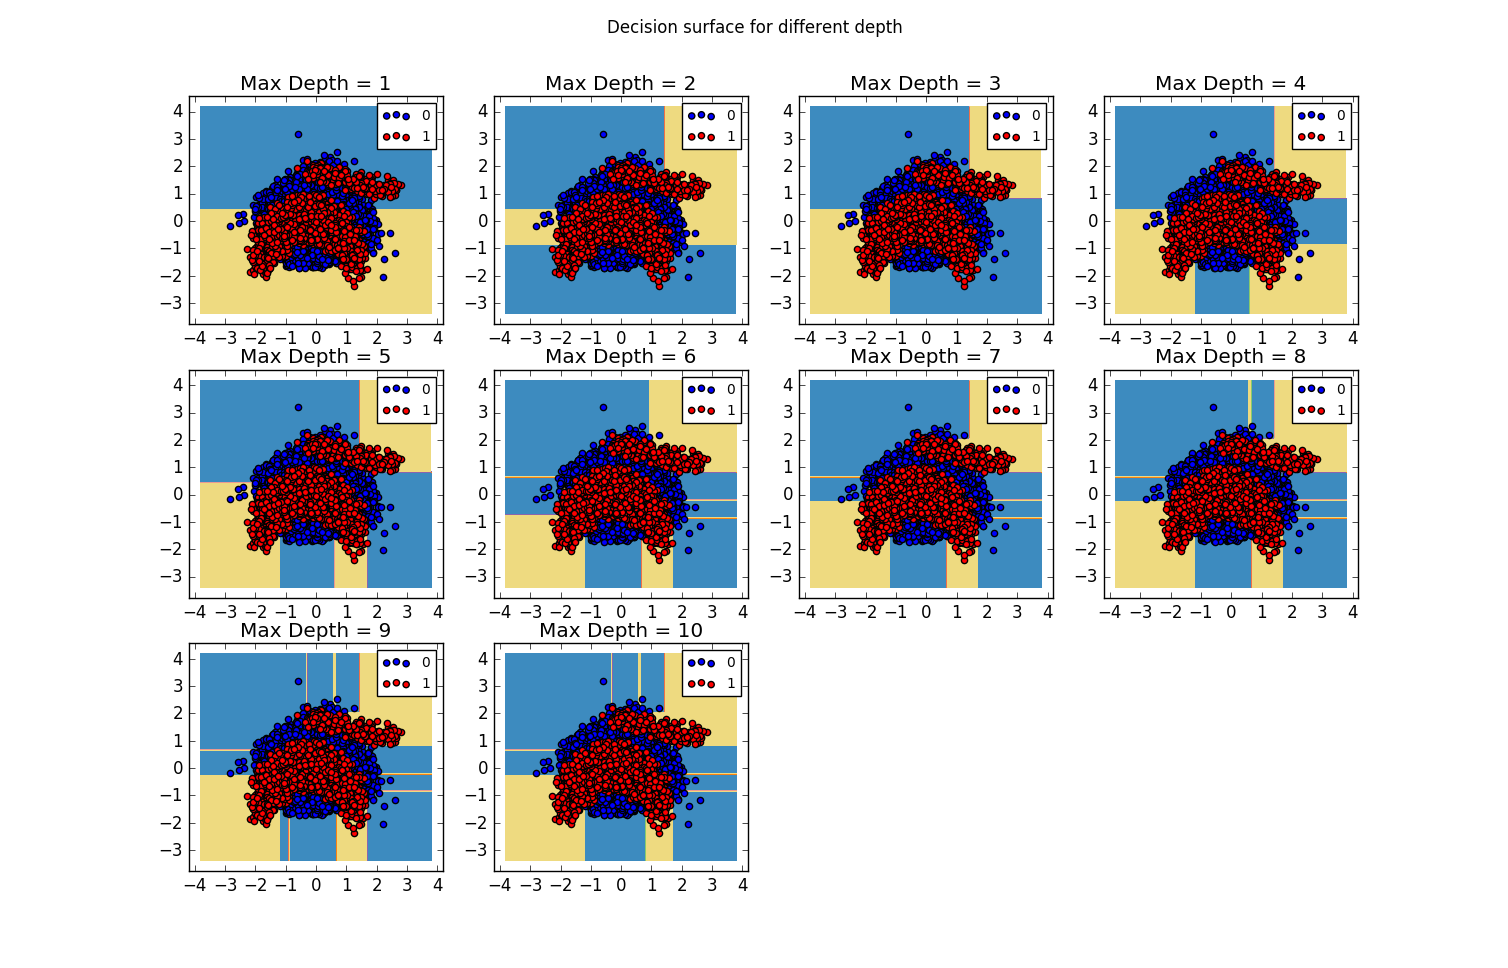
\includegraphics[width = 7.5in]{2_1_2.png}

From the plot we can see that, the decision surface has very little change after max depth = 6.


\begin{sub}{2.1.3}
\end{sub}

\begin{center}
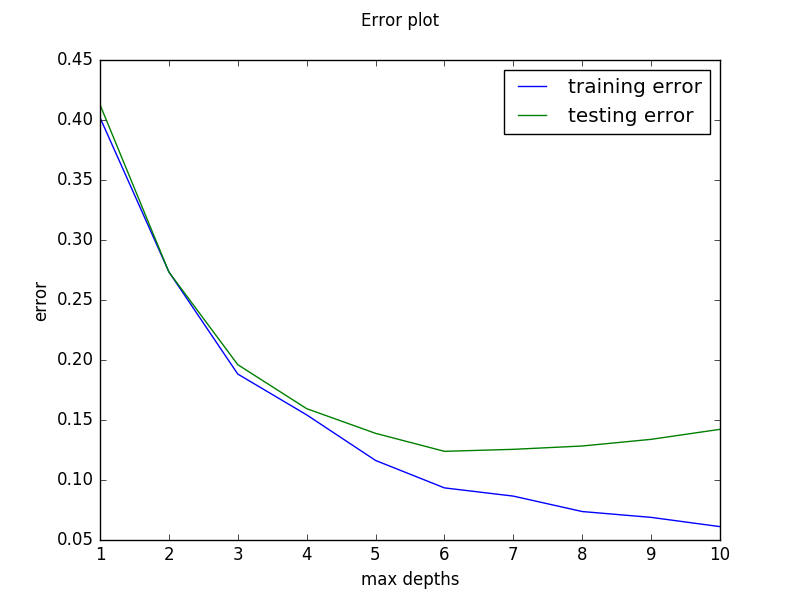
\includegraphics[width = 4in]{2_1_3}
\end{center}

From the plot we see that the model is clearly over-fitting for large max depths. For max depth greater than 6 the testing error is increasing.  

\begin{sub}{2.1.4}
\end{sub}

\begin{minted}{python}
min_error = 1
ite = 0
for a in xrange(1, 21):
    for b in xrange(1, 21):
        for c in xrange(1, 21):
            idx = np.arange(X_train.shape[0])
            np.random.seed(1)
            np.random.shuffle(idx)
            X = X_train[idx]
            y = y_train[idx]

            mean = X.mean(axis=0)
            std = X.std(axis=0)
            X = (X - mean) / std
            #normalize testing data
            X_test_temp = (X_test -mean)/std

            clf = DecisionTreeClassifier(max_depth=a, min_samples_leaf=b,
            		 min_samples_split=c).fit(X, y)

            testing_error = np.sum(np.equal(clf.predict(X_test_temp), 1 - y_test)) /
            		 float(y_test.shape[0])
            if testing_error < min_error:
                min_error = testing_error
                par = [a, b, c]
            ite += 1
>>> min_error
>>> 0.1111111111111
>>> par
>>> [10, 11, 1]
\end{minted}
I searched max depth, min samples leaf, min samples split from 1 to 20, the best testing error is  0.1111111111111, and the corresponding parameters are 10,11 and 1

\section{3 Ada Boost}
\begin{problem}{3.1 Implementation}
\end{problem}

\begin{sub}{3.1.1}
\end{sub}

\begin{minted}{python}
def AdaBoost(X, y,n_round=5,test_x = None,test_y= None,visual = False):
    '''
    :param nd-array X: Training data
    :param 1d-array y: Training labels
    :param int n_round: Number of rounds default = 5
    :param nd-array test_x: Testing data default None
    :param 1d-array test_y: Testing labels default None
    :param Boolean visual: True for visualize default None
    :return: trainining error/ testing error of the Final model  
    '''
    
    n_instance = X.shape[0]
    w = np.ones(n_instance) / n_instance
    models = np.zeros(n_round,dtype = object)
    error = np.zeros(n_round)
    alphas = np.zeros(n_round)

    mean = X.mean(axis=0)
    std = X.std(axis=0)
    X = (X - mean) / std
    

    for n in xrange(1, n_round + 1):
        W = np.sum(w)
        clf = DecisionTreeClassifier(max_depth=3).fit(X,y,sample_weight=w)
        models[n-1] = clf
        error = np.sum((1-np.equal(clf.predict(X), y)) * w)/W
        alphas[n-1] = np.log((1-error)/error)
        w = np.exp((1- np.equal(clf.predict(X),y))*alphas[n-1])*w

        #visualizer
        if visual:
            plot_colors = 'br'
            plt.subplot(2, 5, n)
            x_min, x_max = X[:, 0].min() - 1, X[:, 0].max() + 1
            y_min, y_max = X[:, 1].min() - 1, X[:, 1].max() + 1
            xx, yy = np.meshgrid(np.arange(x_min, x_max, plot_step),
                                 np.arange(y_min, y_max, plot_step))

            Z = np.sum(map(lambda i:alphas[i] * models[i].predict(np.c_[xx.ravel(),
            			 yy.ravel()]),list(xrange(n))),0)
            Z = Z.reshape(xx.shape)
            cs = plt.contourf(xx, yy, Z, cmap=plt.cm.Paired)
            plt.axis("tight")

            for i, color in zip([-1,1], plot_colors):
                idx = np.where(y == i)
                plt.scatter(X[idx, 0], X[idx, 1],s=10000*(w/W) , c=color, 
                			label="class" + str(i), cmap=plt.cm.Paired)
                plt.legend(fontsize=10,title = 'Round' + str(n))
    plt.suptitle('Decision surface for different rounds')
    plt.show()

    # record rounds errors
    G_n = np.array(map(lambda i: alphas[i] * models[i].predict(X), list(xrange(n))))
    train_error = 1 - np.sum(np.equal(np.sign(np.sum(G_n,0)),y))/float(n_instance)

    if  (test_x != None) and  (test_y != None) :
        G_n_test = np.array(map(lambda i: alphas[i] * models[i].predict(test_x),
        			 list(xrange(n))))
        test_error = 1 - np.sum(np.equal(np.sign(np.sum(G_n_test,0)),test_y))/
        			float(test_y.shape[0])
        return [train_error,test_error]

    else:
        return train_error
>>> AdaBoost(X_train,y_train,10,visual = True)
\end{minted}


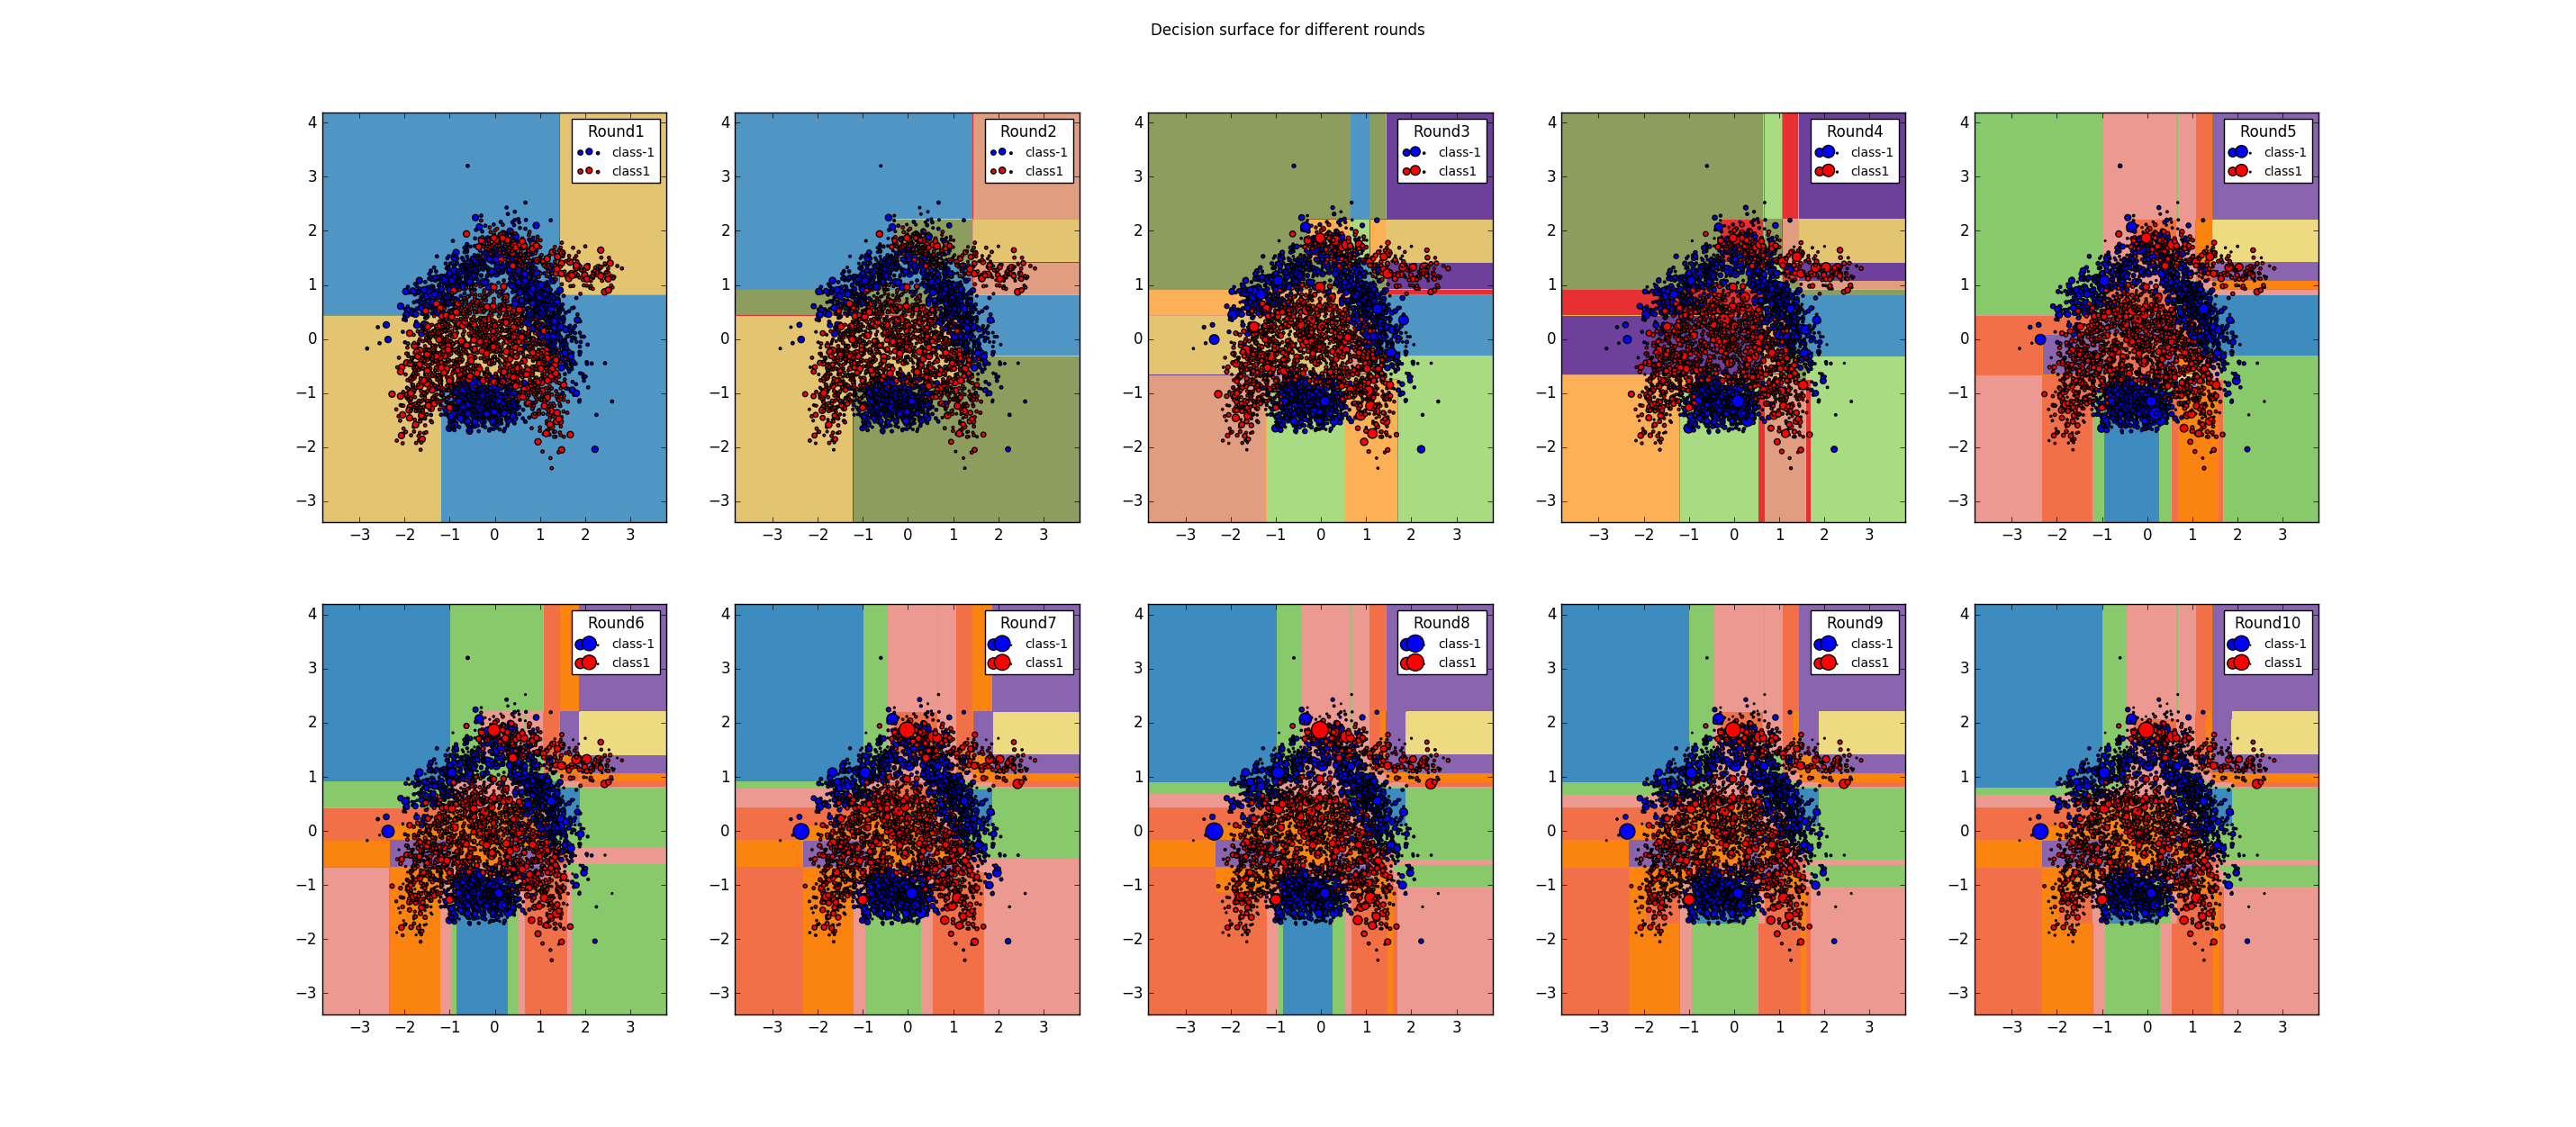
\includegraphics[width = 7in]{3_1_2}

From the plot we can see that some points near the decision surface are getting larger weights with further boosting. 

\begin{sub}{3.1.3}
\end{sub}

\begin{center}
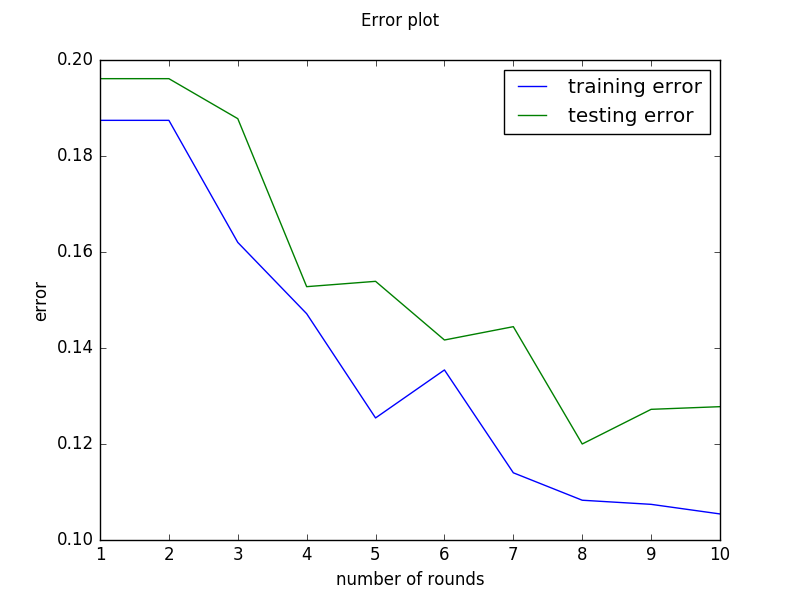
\includegraphics[width = 4in]{3_1_3}
\end{center}

From the plot we see that the both of the training and testing error are decreasing when adding rounds. The over-fitting is not clear yet, so we may try to add more rounds to see how the AdaBoost works on this data set.

\section{4 Gradient Boosting Machines}
\begin{problem}{4.1}
\end{problem} 

For square loss: $l(\hat{y},y) = \frac{1}{2}(\hat{y} - y)^2$\\
From the Gradient Boosting Machines, 
\begin{align}
(g_m)_i &= \frac{\partial}{\partial f(x_i)} \sum_{i=1}^{n}\frac{1}{2}(y_i - f(x_i))^2 \vert_{f(x_i) = f_{m-1}(x_i)}\\
&= \frac{\partial}{\partial f(x_i)} \frac{1}{2}(y_i - f(x_i))^2 \vert_{f(x_i) = f_{m-1}(x_i)}\\
&= -(y_i - f(x_i)) \vert_{f(x_i) = f_{m-1}(x_i)}\\
&= -(y_i - f_{m-1}(x_i))
\end{align}
Then \begin{align}
h_m &=  \underset{h \in \mathcal{F}}{\operatorname{arg min}} \sum_{i=1}^{n} ((-g_m)_i - h(x_i))^2\\
 &=  \underset{h \in \mathcal{F}}{\operatorname{arg min}} \sum_{i=1}^{n} ((y_i - f_{m-1}(x_i)) - h(x_i))^2
\end{align}

\begin{problem}{4.2}
\end{problem}
For logistic loss: $l(m) = ln(1+e^{-m})$\\
From the Gradient Boosting Machines, 
\begin{align}
(g_m)_i &= \frac{\partial}{\partial f(x_i)} \sum_{i=1}^{n}ln(1+ e^{-y_if(x_i)}) \vert_{f(x_i) = f_{m-1}(x_i)}\\
&= \frac{\partial}{\partial f(x_i)} ln(1+ e^{-y_if(x_i)}) \vert_{f(x_i) = f_{m-1}(x_i)}\\
&= \frac{-y_ie^{-y_if(x_i)}}{1+e^{-y_if(x_i)}} \vert_{f(x_i) = f_{m-1}(x_i)} \\
&=  \frac{-y_ie^{-y_if_{m-1}(x_i)}}{1+e^{-y_if_{m-1}(x_i)}}
\end{align}
Then\begin{align}
h_m &=  \underset{h \in \mathcal{F}}{\operatorname{arg min}} \sum_{i=1}^{n} ((-g_m)_i - h(x_i))^2\\
 &=  \underset{h \in \mathcal{F}}{\operatorname{arg min}} \sum_{i=1}^{n} ( \frac{y_ie^{-y_if_{m-1}(x_i)}}{1+e^{-y_if_{m-1}(x_i)}}- h(x_i))^2
\end{align}

\section{5 From Margins to Conditional Probabilities}
\begin{problem}{5.1}
\end{problem}
Since $y\in\{1,-1\}$
\begin{align}
E_y[l(yf(x))|x] &= P(y = -1|x)l(-f(x)) + P(y = 1|x)l(f(x))\\
&= (1- P(y = 1|x))l(-f(x)) + P(y = 1|x)l(f(x))\\
&= (1- \pi(x))l(-f(x)) + \pi(x)l(f(x))
\end{align}

\begin{problem}{5.2}
\end{problem}
For exponential loss $l(y,f(x)) = e^{-yf(x)}$:
\begin{align}
f^* &= \underset{f}{\operatorname{arg min}} \hspace{0.05in} E_y[l(yf(x))|x]\\
&= \underset{f}{\operatorname{arg min}} \hspace{0.05in} (1- \pi(x))e^{f(x)} + \pi(x)e^{-f(x)}
\end{align}
If we take partial derivative of the target function w.r.t f:
\begin{align}
\frac{\partial}{\partial f}  (1- \pi(x))e^{f(x)} + \pi(x)e^{-f(x)} = (1- \pi(x))e^{f(x)} - \pi(x)e^{-f(x)} = 0
\end{align}
We have:
\begin{align}
e^{2f(x)} &= \frac{\pi(x)}{1- \pi(x)}\\
f^*(x) &= f(x) = \frac{1}{2} ln(\frac{\pi(x)}{1- \pi(x)})
\end{align}
On the contrary, if we are given $f^*$, we can solve $\pi(x)$ from eqn(20):
\begin{align}
\frac{1}{2} ln(\frac{\pi(x)}{1- \pi(x)}) &= \frac{1}{2} ln(\frac{1}{1- \pi(x)}-1) = f^*(x)\\
\frac{1}{1-\pi(x)} &= e^{2f^*(x)} +1\\
\pi(x) &= \frac{e^{2f^*(x)}}{e^{2f^*(x)} +1} = \frac{1}{1+e^{-2f^*(x)}}\\
\end{align}

\begin{problem}{5.3}
\end{problem}
For the logistic loss function $l(y,f(x)) = ln(1+e^{-yf(x)})$:
\begin{align}
f^* &= \underset{f}{\operatorname{arg min}} \hspace{0.05in} E_y[l(yf(x))|x]\\
&= \underset{f}{\operatorname{arg min}} \hspace{0.05in} (1- \pi(x))ln(1+e^{f(x)}) + \pi(x)ln(1+e^{-f(x)})
\end{align}
If we take partial derivative of the target function w.r.t f:
\begin{align}
(1-\pi(x))\frac{e^{f(x)}}{1+e^{f(x)}}+\pi(x)\frac{-e^{-f(x)}}{1+e^{-f(x)}})=0
\end{align}
We have:
\begin{align}
\frac{(1-\pi(x)) e^{f(x)}}{1+e^{f(x)}}- \frac{\pi(x)}{e^{f(x)}+1} = 0
\end{align}
Since $e^{f(x)}+1 > 0$:
\begin{align}
 \pi(x) &= (1-\pi(x)) e^{f(x)} \\
f^*(x)&= f(x) = ln(\frac{\pi(x)}{1-\pi(x)})
\end{align}
If we are given $f^*$, we can solve $\pi(x)$ from eqn(30):
\begin{align}
f^*(x) &= ln(\frac{1}{1-\pi(x)}-1)\\
\pi(x) &= 1-\frac{1}{e^{f^*(x)}+1}\\
&= \frac{e^{f^*(x)}}{e^{f^*(x)}+1}\\
&= \frac{1}{1+e^{-f^*(x)}}
\end{align}

\begin{problem}{5.4}
\end{problem}
For the hinge loss $l(y,f(x)) = max(0,1-yf(x))$:
\begin{align}
f^* &= \underset{f}{\operatorname{arg min}} \hspace{0.05in} E_y[l(yf(x))|x]\\
&= \underset{f}{\operatorname{arg min}} \hspace{0.05in} (1- \pi(x))max(0,1+f(x)) + \pi(x)max(0,1-f(x))\\
& = \underset{f}{\operatorname{arg min}} \hspace{0.05in} F
\end{align} 
i) if $f \leq -1$:
\begin{align}
F = &\pi(x) (1-f(x)) \\
\frac{\partial F}{\partial f}&= -\pi(x) <0
\end{align} 
The function F is decreasing, therefore to minimize F we choose $f^*(x)$ = -1\\
ii) if $f \geq 1$:
\begin{align}
F = (& 1-\pi(x)) (1+f(x)) \\
\frac{\partial F}{\partial f}&= 1-\pi(x) >0
\end{align} 
The function F is increasing, therefore to minimize F we choose $f^*(x)s$ 1\\
iii) if $-1 \leq f \leq 1$:
\begin{align}
F = (1-\pi(x)) &(1+f(x)) +   \pi(x) (1-f(x))  \\
\frac{\partial F}{\partial f}&= 1-2\pi(x)
\end{align}
For $\pi(x)\leq \frac{1}{2}$, $\frac{\partial F}{\partial f} \geq 0 $, the function is increasing, then we choose $f^*(x) = -1$ \\
For $\pi(x)\geq \frac{1}{2}$, $\frac{\partial F}{\partial f} \leq 0 $, the function is decreasing, then we choose $f^*(x) = 1$ \\
From above it's equivalent to $f^*(x) = sign(\pi(x)-\frac{1}{2})$
\end{document}
